\chapter{Evaluation}
\label{c:evaluation}


The aim of this study is to understand the characteristics and user preferences for each of our three keyboard prototypes. We conducted a user study consisting of text-copy tasks using sentences sampled from the NUS SMS corpus compiled by Chen, et al. \cite{Chen2013} which consists of more than 30,000 Chinese short messages from Chinese users from all over China and is publicly available\footnote{https://github.com/kite1988/nus-sms-corpus}.
For our study, we only consider short messages from users living in Beijing who are known to speak the most standard dialect of Mandarin Chinese, in order to ensure that participants in our study are not confronted with unfamiliar local expressions or idioms. To focus only on Chinese sentences, we further restrict the study to samples that contain between 5 and 15 Chinese characters and no Latin letters or punctuation symbols.




\section{Participants}
We recruited 15 participants between the ages of 20 to 35 (\textit{M} = 25.9, \textit{SD} = 4.5) from various departments at our university and a nearby language training institution. 8 are native speakers of Chinese and 7 are highly proficient language students. 14 are right-handed and 1 is left-handed. All of them chose to wear the smartwatch on the wrist of their non-dominant hand and typed with the index finger of their dominant hand. 12 had never used a smartwatch before, the remaining 3 only for a short amount of time. All participants were very familiar with Chinese text entry using the standard QWERTY keyboard layout with the Pinyin system. Each participant was paid the equivalent of USD 5 in compensation for their time.





\section{Procedure}
Participants were seated in a quiet environment and were asked to rest their arm on the table in front of them to avoid fatigue. A computer screen in front of the participant instructed the participant which keyboard to use and what sentences to type. Figure \ref{fig:figure4} shows our user study setup. Participants were given a chance to experiment with each keyboard before starting the trials.







\begin{figure}
  \centering
  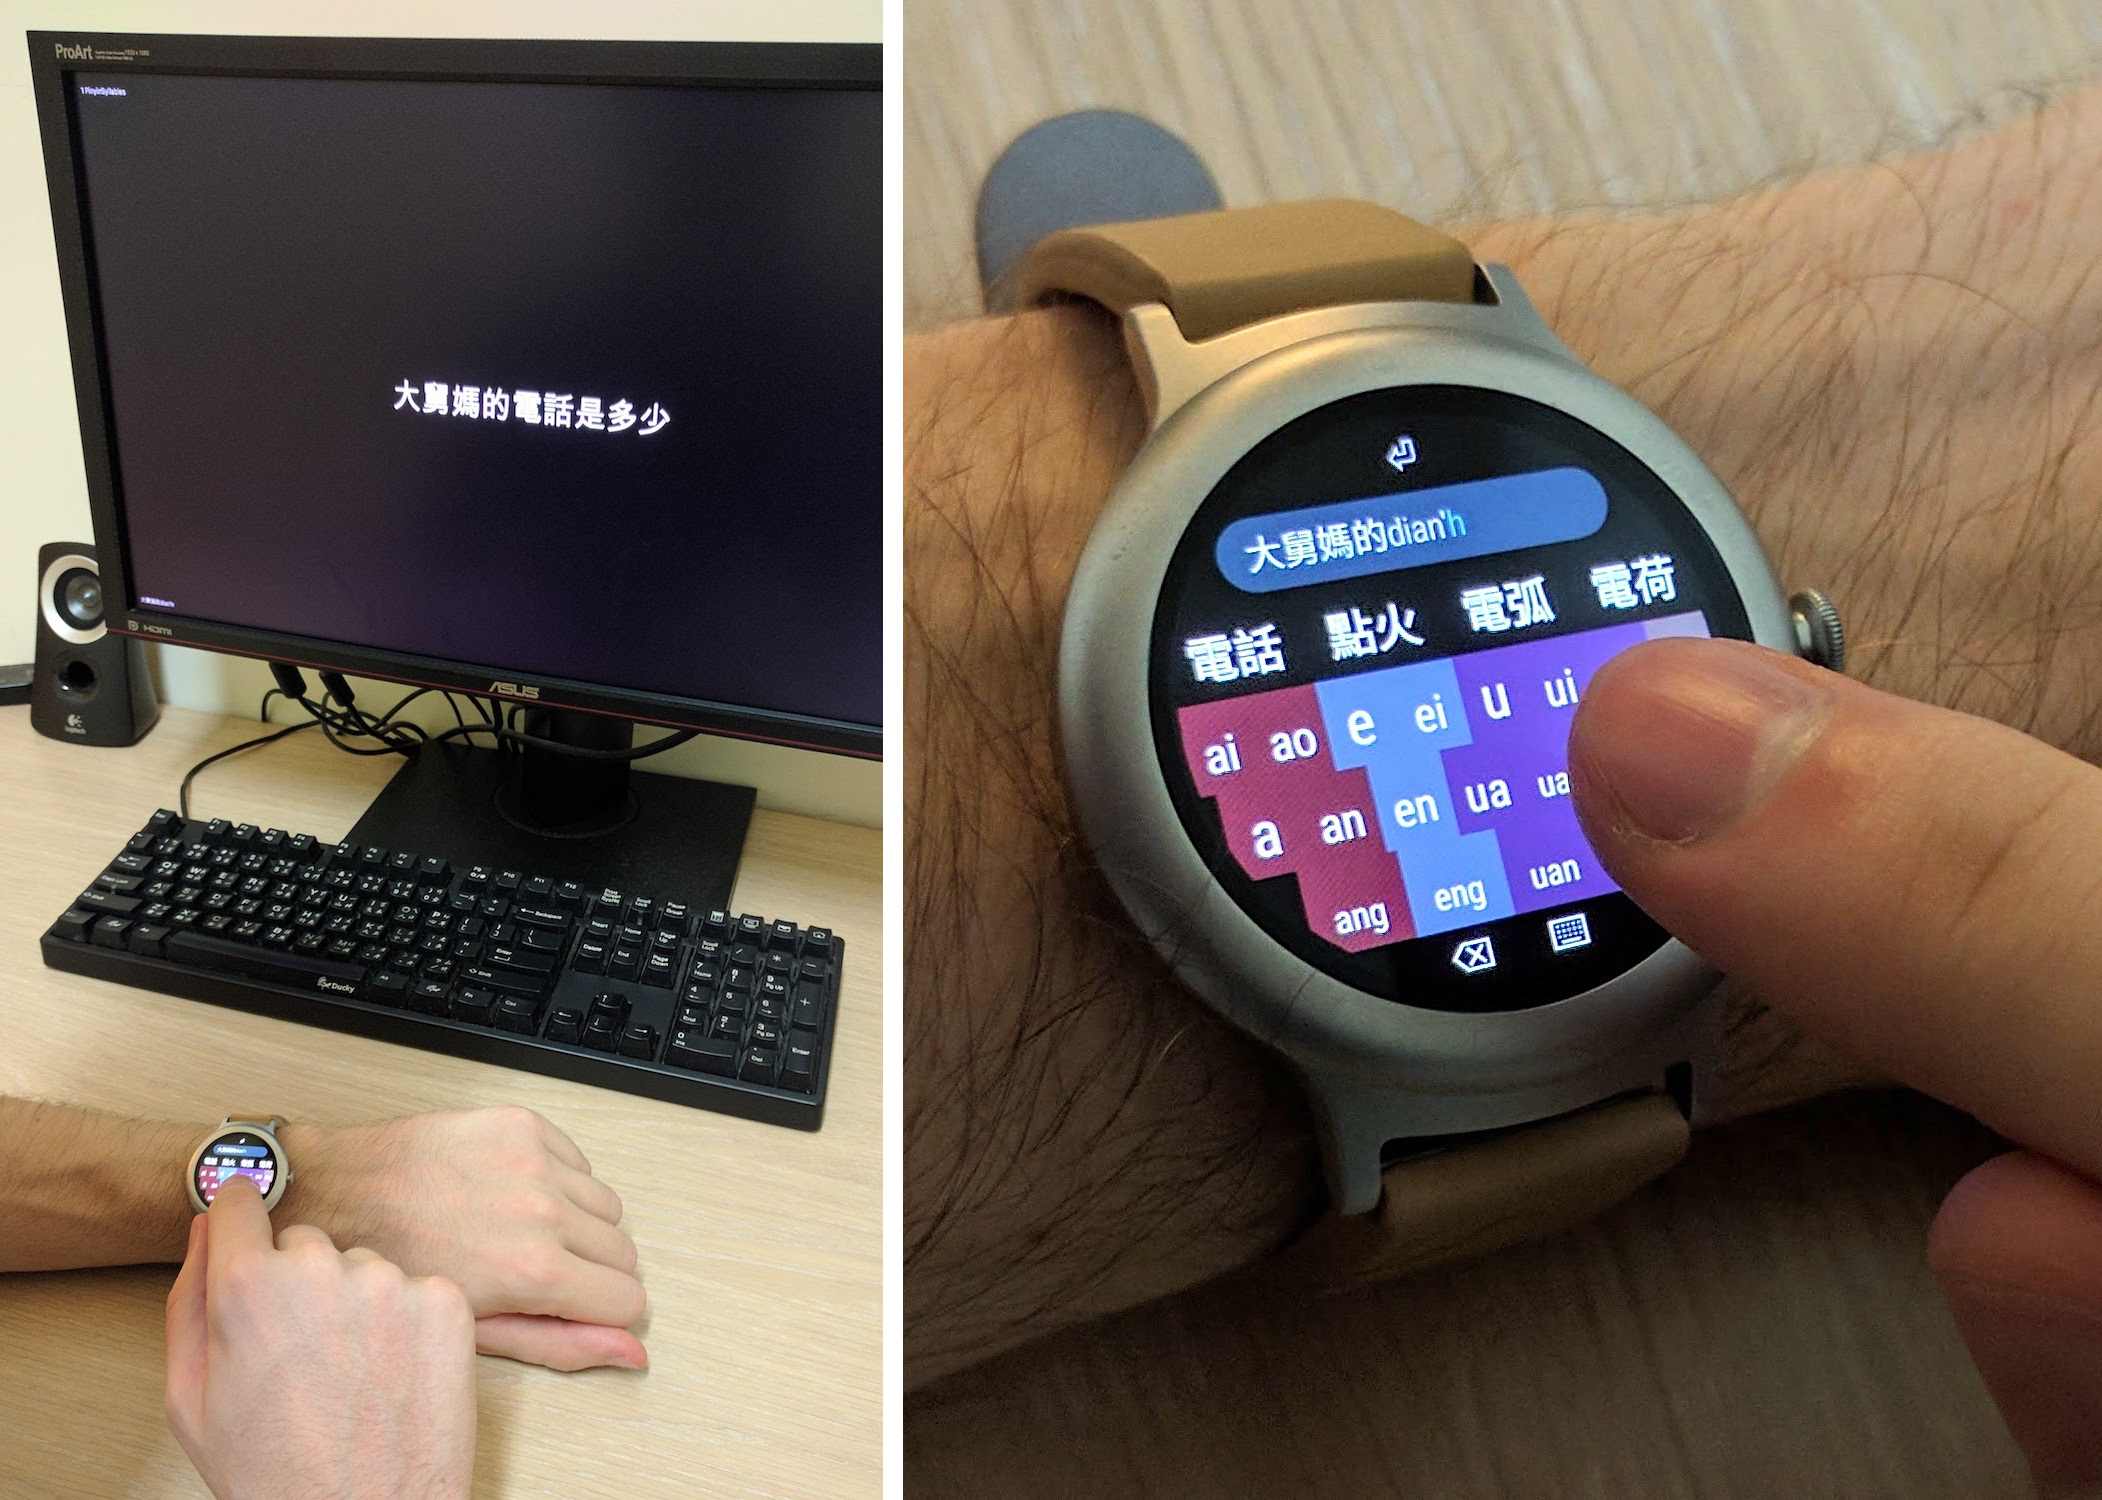
\includegraphics[width=1\columnwidth]{figures/user_study_setup}
  \caption{The setup of our user study.}~\label{fig:figure4}
\end{figure}








For each of the three keyboards, participants had to enter 25 sentences. The total of 3 $\times$ 25 = 75 sentences for all keyboard prototypes was randomly sampled from a specific subset of the NUS SMS corpus \cite{Chen2013} as explained above. These sentences contain only Chinese characters. All participants entered the same 75 sentences in the same order but the keyboard that was used for the first, second and third block of 25 sentences varied for each participant. We used Latin square design to counterbalance the order of keyboards.

Participants were asked to type as fast and as accurately as possible. For each sentence, before pressing the first key, participants were allowed to rest and memorize the sentence displayed on the computer screen in front of them for as long as they wanted. After entering each sentence, participants would press the ENTER key to continue to the next sentence.

After completing all trials, users were asked to rate each keyboard on a 5-point Likert scale and comment on positive and negative aspects of each keyboard.








\section{Results}
During the trials, we recorded 1,125 samples of sentence input representing close to 30,000 individual input events and 8.3 hours of non-stop typing data.


\begin{table}[]
\renewcommand{\arraystretch}{1.7}
\centering
\caption{Mean Chinese Characters per Minute (CCPM), Keystrokes per Chinese Character (KSPCC), Total Error Rate (TER) and Used Bandwidth (UBW) for each keyboard prototype. SDs are in parenthesis.}
\label{table:CCPM_KSPCC_TER_UBW}
\begin{tabular}{llll}

      & Growing Finals & Pinyin Syllables & QWERTY          \\ \hline
CCPM  & 19.39 (7.1)    & 18.51 (7.4)      & 22.39 (10.0)    \\
KSPCC & 3.72 (1.1)     & 2.98 (0.9)       & 3.79 (1.4)      \\
TER   & 7.72 (7.3)     & 9.49 (8.0)       & 12.21 (8.0)     \\
UBW   & 86.84 (11.8)   & 84.08 (12.2)     & 79.45 (12.6)    \\ \hline
\end{tabular}
\end{table}






\section{Text Entry Performance}
We measure text entry speed in Chinese characters per minute (CCPM) that we calculate as follows:

\[ CCPM = \frac{|C|}{T} \times 60 \]

where |\textit{C}| is the number of Chinese characters in the transcribed text and \textit{T} is the elapsed time in seconds from the first button press to the selection of the last Chinese character candidate before pressing ENTER.





In our study, the standard QWERTY keyboard slightly outperforms Growing Finals and Pinyin Syllables in terms of text entry speed (Table \ref{table:CCPM_KSPCC_TER_UBW}) with 22.4 CCPM (\textit{SD} = 10) but the high standard deviation indicates that it works better for some participants than others. Growing Finals offers the most stable input speed at 19.4 CCPM (\textit{SD} = 7) and Pinyin Syllables reached 18.5 CCPM (\textit{SD} = 7.5) on average despite steep learning curve.


\section{Error Rate}
We calculate the total error rate (TER) as described by Soukoreff et al \cite{Soukoreff:2003:MTE:642611.642632} that accounts for corrected and uncorrected errors. Considering the unique input characteristics of entering Chinese characters using Pinyin and candidate selections, we reinterpret the original formula for TER as follows:

\[ TER = \frac{E + D}{K + S + E + D} \]

where \textit{E} refers to the Levenshtein distance between the transcribed Chinese characters and the given sentence. \textit{D} refers to the number of DELETE events which may either delete the previously entered Latin Pinyin letter during Chinese character composition or a Chinese character after a Chinese character has been selected. \textit{K} and \textit{S} refer to key events for entering Latin Pinyin letters or selection events for converting Pinyin to Chinese characters respectively.


Due to the enlarged key size in many input states, Growing Finals and Pinyin Syllables have a lower TER of 7.7\% (\textit{SD} = 7.3) and 9.5\% (\textit{SD} = 8) respectively. Text entry on tiny QWERTY keyboards is feasible when carefully typing letter by letter but still error prone on small smartwatch devices \cite{Leiva:2015:TET:2702123.2702388}. The TER of 12.2\% (\textit{SD} = 8) reflects this fact.


\section{Keystrokes per Chinese Character}
Unlike Latin languages such as English, when entering Chinese characters using the Pinyin system, a single keystroke will not represent a single Chinese character entered, rather a sequence of keystrokes and candidate selections will eventually lead to one or more Chinese characters being entered. We compute keystroke per Chinese character (KSCC) as follows:
\[ KSPCC = \frac{K + S + D}{|C|} \]
where \textit{K}, \textit{S} and \textit{D} refer to key, selection or delete events and |\textit{C}| refers to the number of Chinese characters in the transcribed sentence.

Pinyin Syllables has the lowest and most stable KSCC at 3 (\textit{SD} = 0.9) because each pinyin syllable can be entered with a fixed number of 2 key press events, which means that higher input speeds can be expected once users fully memorize key locations and spend less time on visual search. The letter-by-letter input mechanics that Growing Finals and Standard QWERTY have in common leads to similar KSPCC values of 3.72 (\textit{SD} = 1.1) and 3.79 (\textit{SD} = 1.4) respectively.
 
 
 
 \begin{figure}
  \centering
  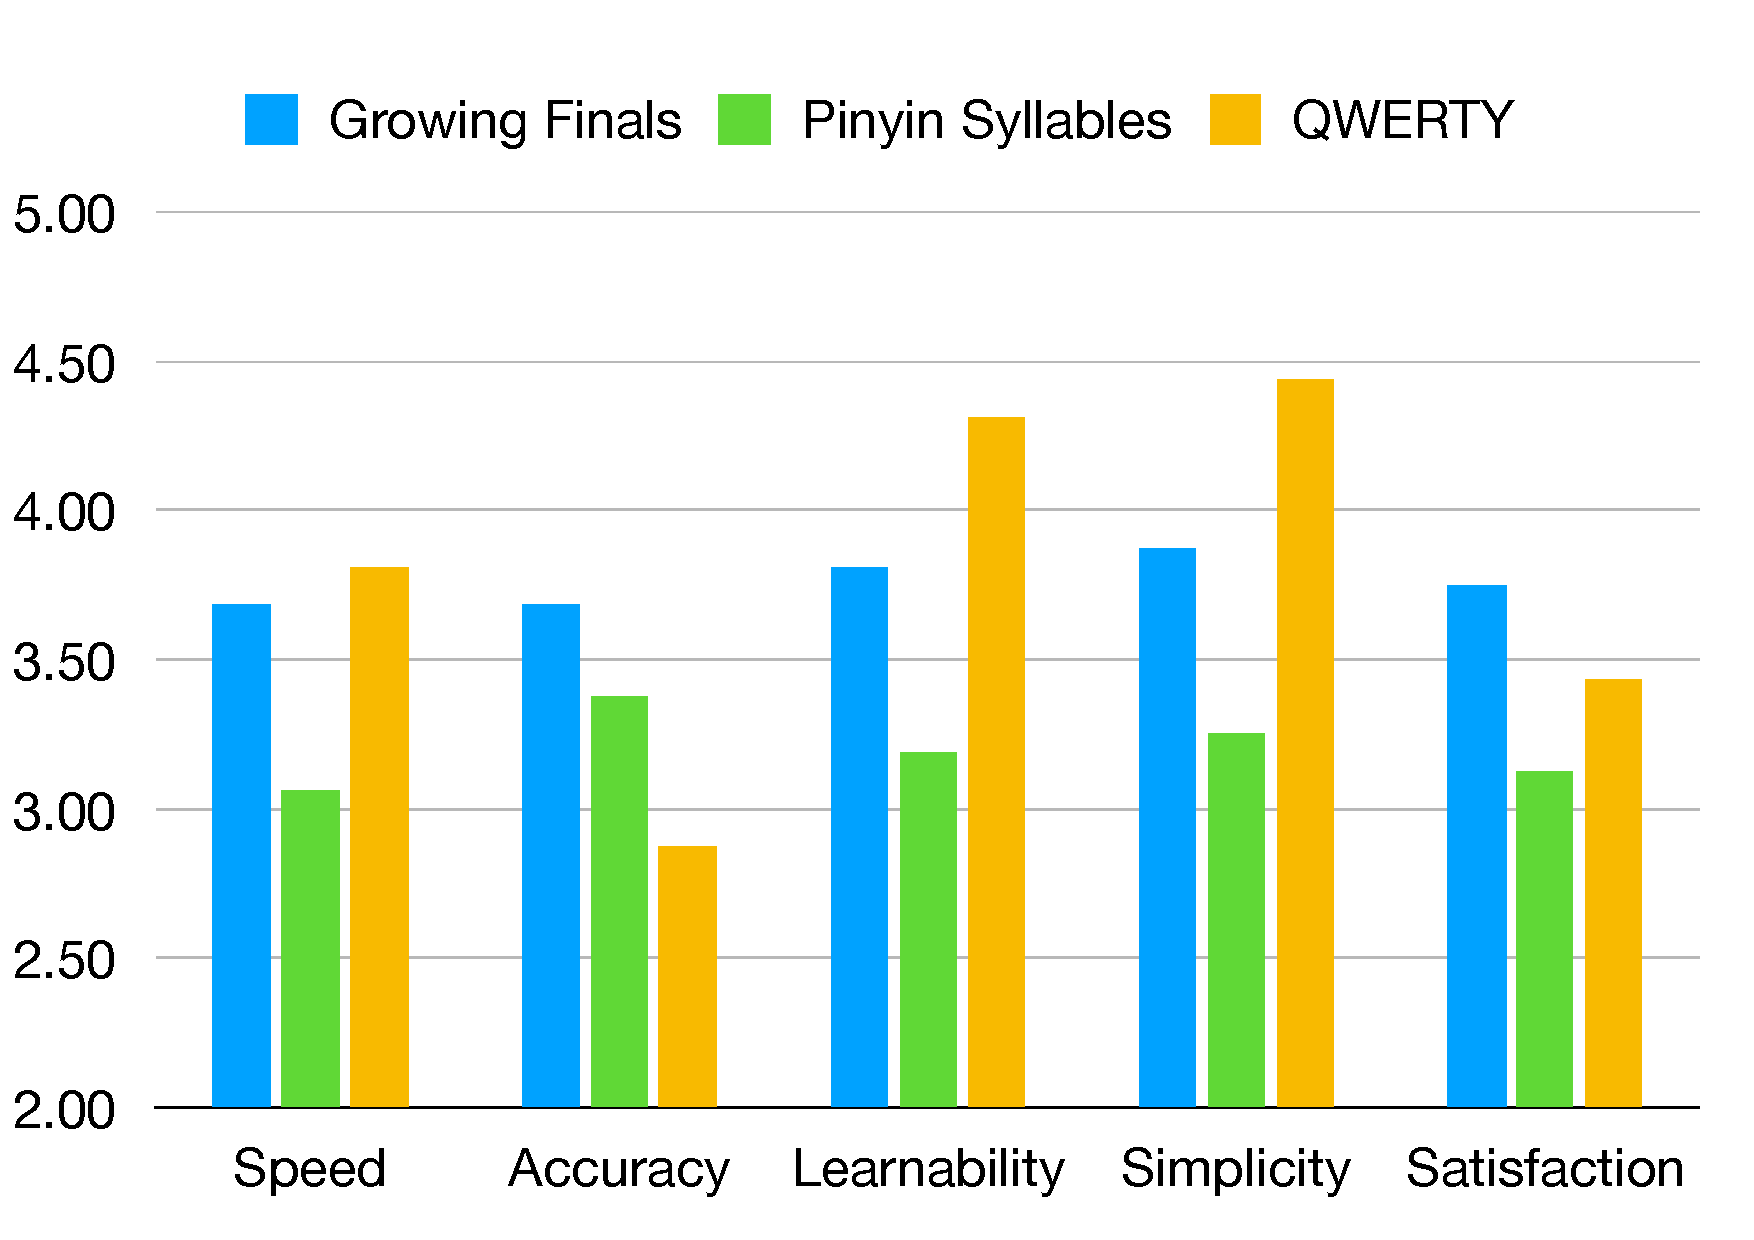
\includegraphics[width=1\columnwidth]{figures/user_prefs}
  \caption{Subjective user feedback for each keyboard prototype on a 5-point Likert scale.}~\label{fig:figure5}
\end{figure}

 
 

\section{Utilized Bandwidth}
As suggested by Soukoreff, et al. \cite{Soukoreff:2003:MTE:642611.642632} we calculate the Utilized Bandwidth (UBW) as a measure of what percentage of input events lead up to the final transcribed text and what percentage of input events are wasted on errors and correcting errors:

\[ UBW = \frac{K + S}{K + S + E + D \times 2} \]

where \textit{D} refers to the number of delete events. \textit{D} is counted twice because every delete event will undo a previously performed key event. The UBW is 100\% if no errors are made and the delete key is never used. The high UBW of 87\% (\textit{SD} = 12) of Growing Finals indicates that the delete key was necessary less often compared to other keyboard prototypes.





\section{User Preference}
Figure \ref{fig:figure5} shows the subjective user feedback. Growing Finals and QWERTY lead in terms of perceived input speed and Growing Finals and Pinyin Syllables lead in terms of typing accuracy. Overall, users were most satisfied with the Growing Finals input method.
Based on the interviews following our study, we found that more than half of our participants preferred either Growing Finals or Pinyin Syllables (Figure \ref{fig:figure6}) despite slightly lower input performance overall. Most participants where more comfortable with Growing Finals because it is similar to the familiar QWERTY layout, however some participants pointed out that Pinyin Syllables might work better for them given more time to practice and become more familiar with all the adaptive layout states.



\begin{figure}
  \centering
  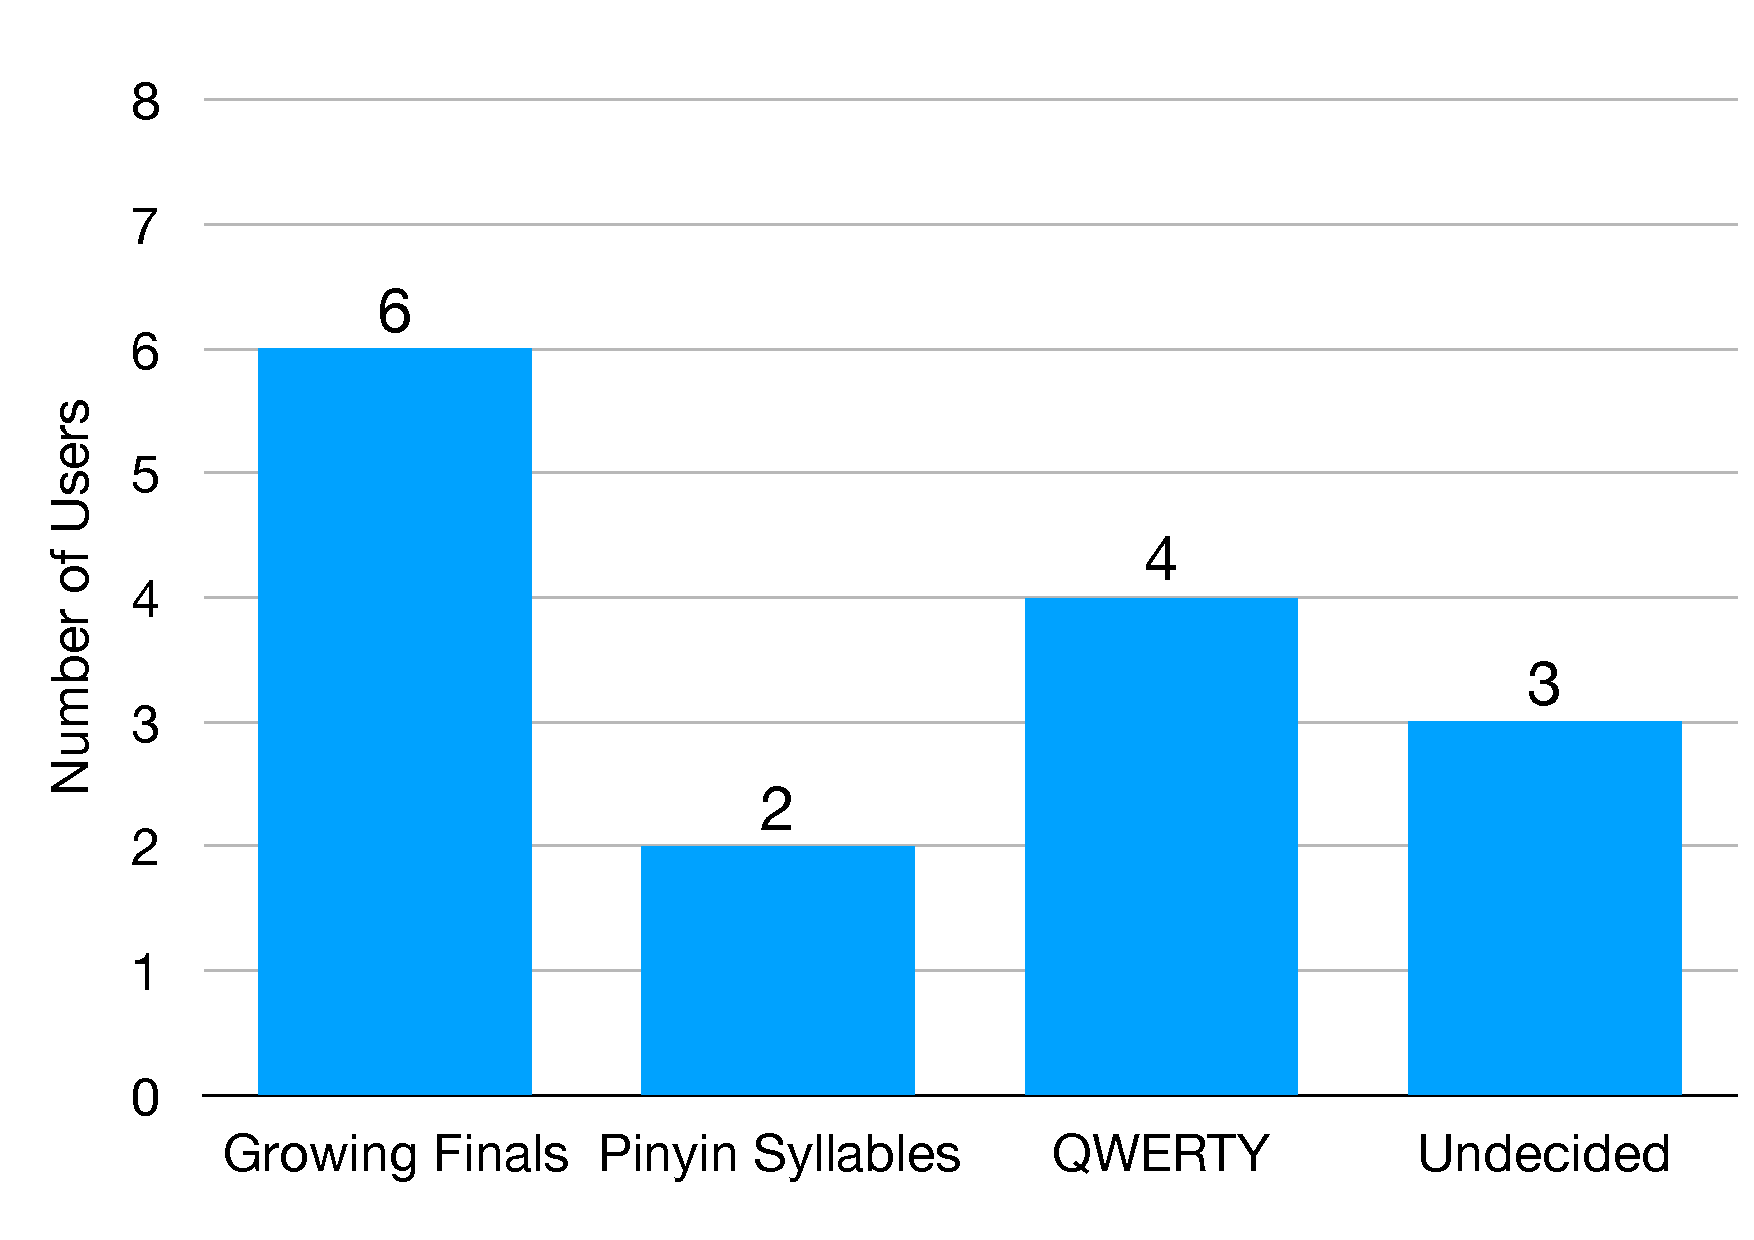
\includegraphics[width=1\columnwidth]{figures/ime_prefs}
  \caption{Preferred keyboard prototype by number of users.}~\label{fig:figure6}
\end{figure}



